

\begin{figure}[H]
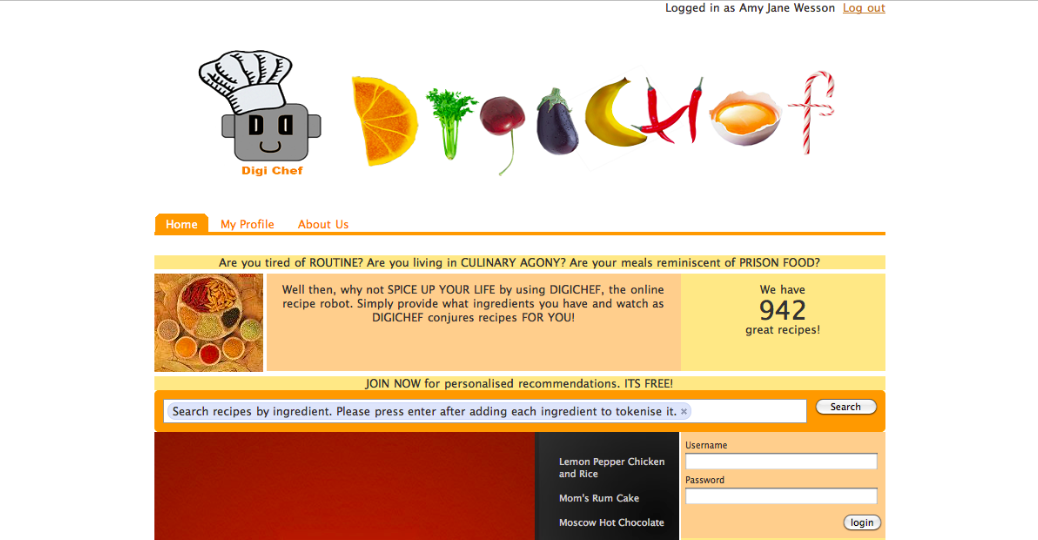
\includegraphics[width=1\textwidth]{result_index}
\caption{Homepage}
\label{fig:result_index}
\end{figure}

As mentioned, white and orange are the colours of choice, along with an appealing logo. The design is effective in meeting the needs of version 2. A search box is ready for search instead of the three drop-down boxes in version 1. And there is a "sign in" box for users to log in. 

\begin{figure}[H]
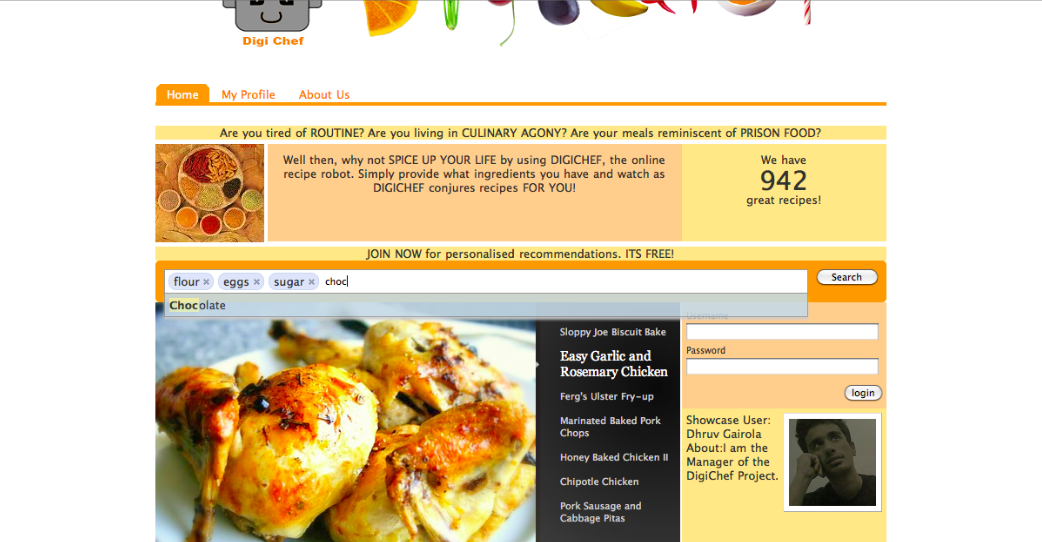
\includegraphics[width=1\textwidth]{result_index2}
\caption{Homepage}
\label{fig:result_index2}
\end{figure}

Figure~\ref{fig:result_index2} donates the results of the JavaScripts slideshow, the auto complete search box, and the user of the week. Notice the recipe name on the right hand side of the slideshow, clicking these generates the image of that recipe in the left part of the slideshow. The image, moreover, links to the exact recipe page. 

\begin{figure}[H]
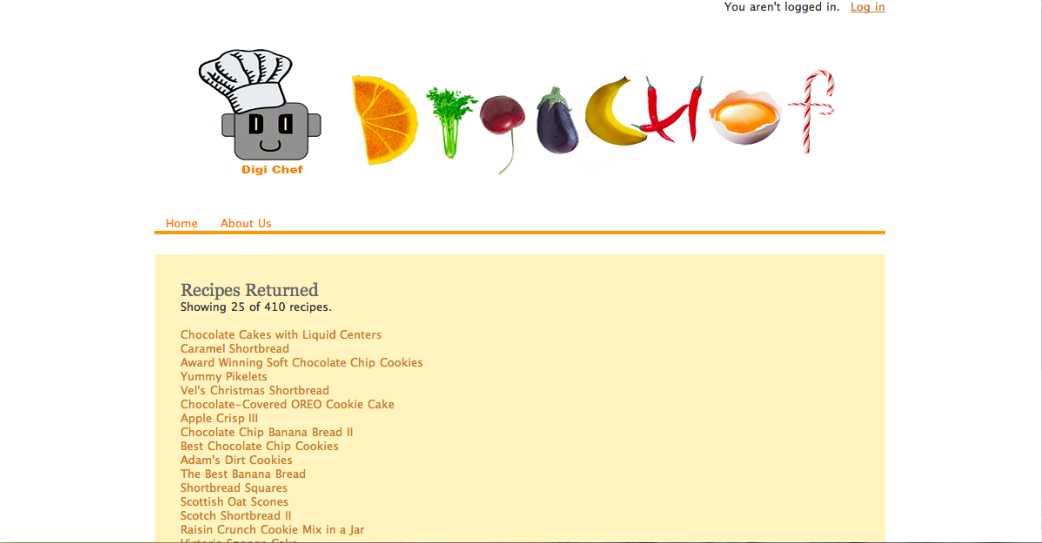
\includegraphics[width=1\textwidth]{result_list}
\caption{Search Result}
\label{fig:result_list}
\end{figure}

Figure~\ref{fig:result_list} shows a recipe list which was generated based on the ingredients entered by the users.

\begin{figure}[H]
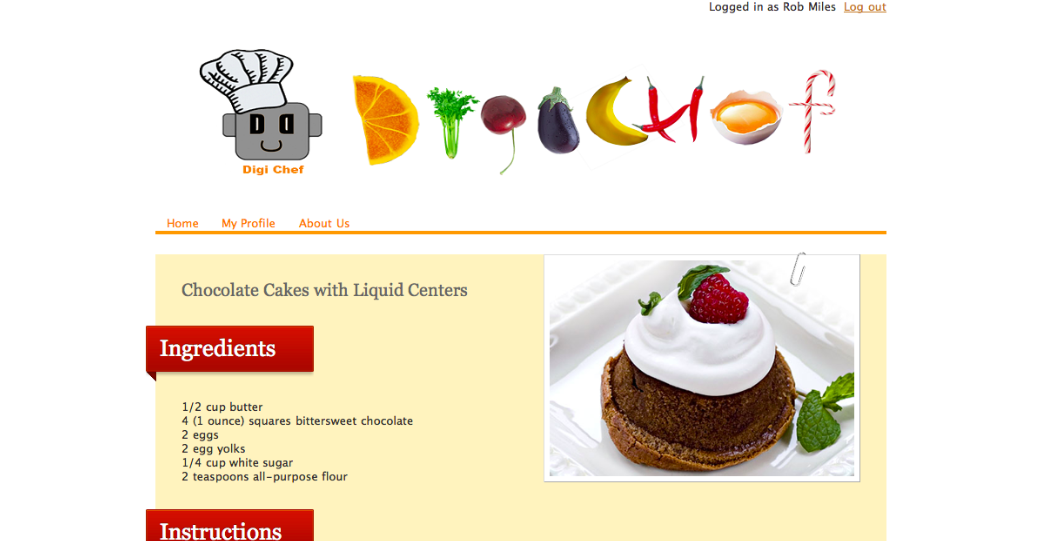
\includegraphics[width=1\textwidth]{result_recipe}
\caption{Recipe Page}
\label{fig:result_recipe}
\end{figure}

\begin{figure}[H]
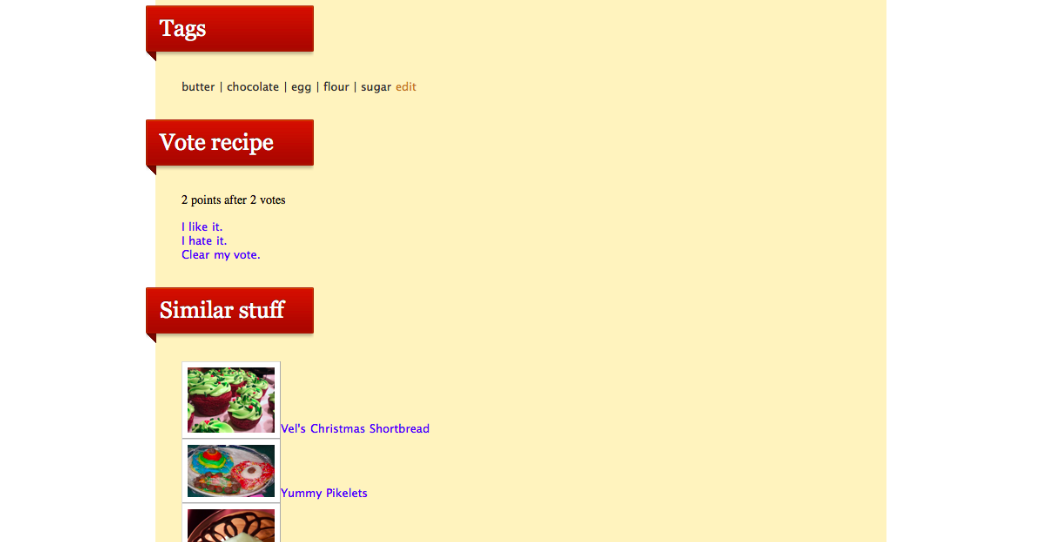
\includegraphics[width=1\textwidth]{result_recipe2}
\caption{Recipe Page}
\label{fig:result_recipe2}
\end{figure}

Figure~\ref{fig:result_recipe} and Figure~\ref{fig:result_recipe2} shows what the version 2 recipe page would like. In Figure~\ref{fig:result_recipe2} we can see that, the design has already simply meets the needs for version 2. In the recipe page, some other related recipes are recommended to the users. The uses can even vote the recipe, moreover, once they have logged in. And all the users (include the unlog-in users) can view the recipe point. 

\begin{figure}[H]
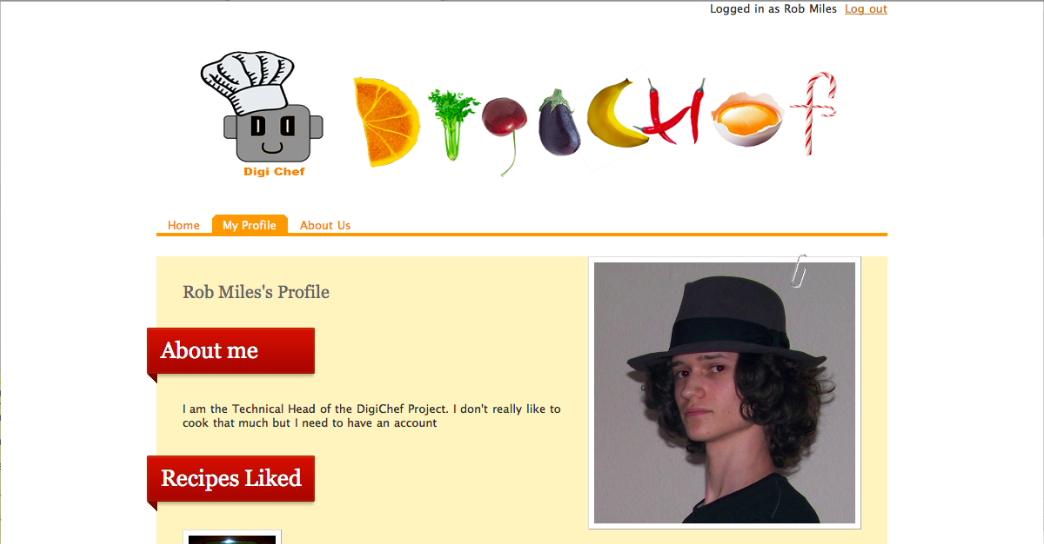
\includegraphics[width=1\textwidth]{result_profile}
\caption{Profile Page}
\label{fig:result_profile}
\end{figure}

Figure~\ref{fig:result_profile} generates the result of how the user profile page would like. There is a simple description about the user. And below this section these is a list of recipes the user liked. 

\begin{figure}[H]
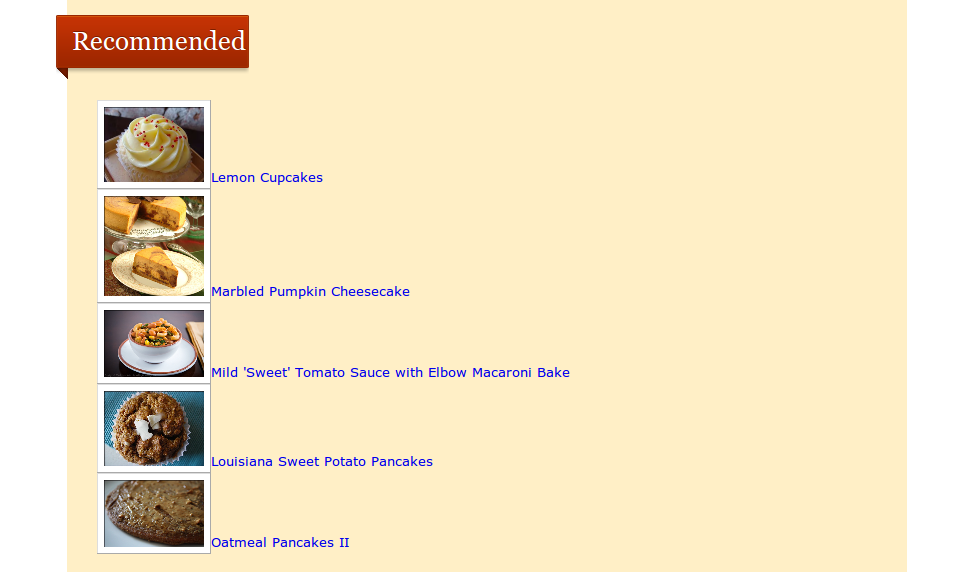
\includegraphics[width=1\textwidth]{recommendations}
\caption{Profile Page}
\label{fig:recommendations}
\end{figure}

Figure~\ref{fig:recommendations} shows the outcome of the recommendation. The "Recommend" section shows a list of recipes automatically generates by the system based on the collaborative filtering algorithm. This list is based on users' vote history and the other users' history if they have same interest with the user.

